% This file was created with tikzplotlib v0.10.1.
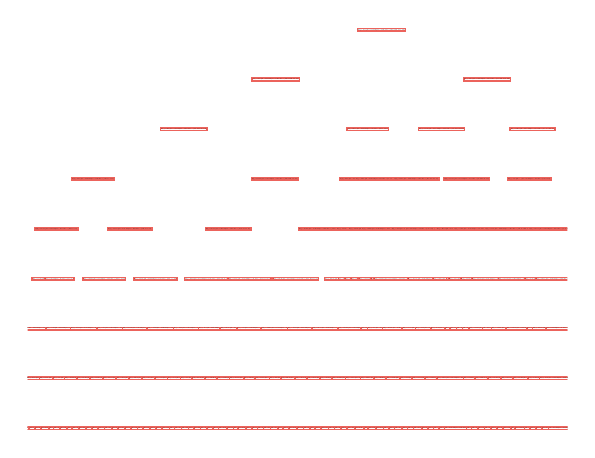
\begin{tikzpicture}

\definecolor{darkgray176}{RGB}{176,176,176}
\definecolor{tomato2369992}{RGB}{236,99,92}

\begin{axis}[
hide x axis,
hide y axis,
tick align=outside,
tick pos=left,
x grid style={darkgray176},
xmin=0, xmax=1,
xtick style={color=black},
y grid style={darkgray176},
ymin=0, ymax=1,
ytick style={color=black}
]
\draw (axis cs:0.00591715976331361,0.0555555555555556) node[
  scale=0.05,
  fill=white,
  draw=tomato2369992,
  line width=0.6pt,
  inner sep=3.6pt,
  text=black,
  rotate=0.0,
  align=center
]{gini = 0.023
samples = 2078
value = [2054, 1, 0, 23]};
\draw (axis cs:0.0177514792899408,0.0555555555555556) node[
  scale=0.05,
  fill=white,
  draw=tomato2369992,
  line width=0.6pt,
  inner sep=3.6pt,
  text=black,
  rotate=0.0,
  align=center
]{gini = 0.064
samples = 425
value = [411, 0, 0, 14]};
\draw (axis cs:0.029585798816568,0.0555555555555556) node[
  scale=0.05,
  fill=white,
  draw=tomato2369992,
  line width=0.6pt,
  inner sep=3.6pt,
  text=black,
  rotate=0.0,
  align=center
]{gini = 0.375
samples = 20
value = [15, 0, 0, 5]};
\draw (axis cs:0.0414201183431953,0.0555555555555556) node[
  scale=0.05,
  fill=white,
  draw=tomato2369992,
  line width=0.6pt,
  inner sep=3.6pt,
  text=black,
  rotate=0.0,
  align=center
]{gini = 0.086
samples = 134
value = [128, 0, 0, 6]};
\draw (axis cs:0.0532544378698225,0.0555555555555556) node[
  scale=0.05,
  fill=white,
  draw=tomato2369992,
  line width=0.6pt,
  inner sep=3.6pt,
  text=black,
  rotate=0.0,
  align=center
]{gini = 0.175
samples = 166
value = [150, 1, 0, 15]};
\draw (axis cs:0.0650887573964497,0.0555555555555556) node[
  scale=0.05,
  fill=white,
  draw=tomato2369992,
  line width=0.6pt,
  inner sep=3.6pt,
  text=black,
  rotate=0.0,
  align=center
]{gini = 0.0
samples = 21
value = [21, 0, 0, 0]};
\draw (axis cs:0.0769230769230769,0.0555555555555556) node[
  scale=0.05,
  fill=white,
  draw=tomato2369992,
  line width=0.6pt,
  inner sep=3.6pt,
  text=black,
  rotate=0.0,
  align=center
]{gini = 0.047
samples = 462
value = [451, 1, 0, 10]};
\draw (axis cs:0.0887573964497041,0.0555555555555556) node[
  scale=0.05,
  fill=white,
  draw=tomato2369992,
  line width=0.6pt,
  inner sep=3.6pt,
  text=black,
  rotate=0.0,
  align=center
]{gini = 0.115
samples = 163
value = [153, 0, 0, 10]};
\draw (axis cs:0.100591715976331,0.0555555555555556) node[
  scale=0.05,
  fill=white,
  draw=tomato2369992,
  line width=0.6pt,
  inner sep=3.6pt,
  text=black,
  rotate=0.0,
  align=center
]{gini = 0.472
samples = 21
value = [8, 0, 0, 13]};
\draw (axis cs:0.112426035502959,0.0555555555555556) node[
  scale=0.05,
  fill=white,
  draw=tomato2369992,
  line width=0.6pt,
  inner sep=3.6pt,
  text=black,
  rotate=0.0,
  align=center
]{gini = 0.351
samples = 955
value = [741, 6, 1, 207]};
\draw (axis cs:0.124260355029586,0.0555555555555556) node[
  scale=0.05,
  fill=white,
  draw=tomato2369992,
  line width=0.6pt,
  inner sep=3.6pt,
  text=black,
  rotate=0.0,
  align=center
]{gini = 0.467
samples = 320
value = [201, 0, 0, 119]};
\draw (axis cs:0.136094674556213,0.0555555555555556) node[
  scale=0.05,
  fill=white,
  draw=tomato2369992,
  line width=0.6pt,
  inner sep=3.6pt,
  text=black,
  rotate=0.0,
  align=center
]{gini = 0.332
samples = 57
value = [45, 0, 0, 12]};
\draw (axis cs:0.14792899408284,0.0555555555555556) node[
  scale=0.05,
  fill=white,
  draw=tomato2369992,
  line width=0.6pt,
  inner sep=3.6pt,
  text=black,
  rotate=0.0,
  align=center
]{gini = 0.255
samples = 314
value = [267, 0, 0, 47]};
\draw (axis cs:0.159763313609467,0.0555555555555556) node[
  scale=0.05,
  fill=white,
  draw=tomato2369992,
  line width=0.6pt,
  inner sep=3.6pt,
  text=black,
  rotate=0.0,
  align=center
]{gini = 0.127
samples = 456
value = [425, 0, 1, 30]};
\draw (axis cs:0.171597633136095,0.0555555555555556) node[
  scale=0.05,
  fill=white,
  draw=tomato2369992,
  line width=0.6pt,
  inner sep=3.6pt,
  text=black,
  rotate=0.0,
  align=center
]{gini = 0.257
samples = 129
value = [110, 1, 2, 16]};
\draw (axis cs:0.183431952662722,0.0555555555555556) node[
  scale=0.05,
  fill=white,
  draw=tomato2369992,
  line width=0.6pt,
  inner sep=3.6pt,
  text=black,
  rotate=0.0,
  align=center
]{gini = 0.467
samples = 70
value = [44, 0, 0, 26]};
\draw (axis cs:0.195266272189349,0.0555555555555556) node[
  scale=0.05,
  fill=white,
  draw=tomato2369992,
  line width=0.6pt,
  inner sep=3.6pt,
  text=black,
  rotate=0.0,
  align=center
]{gini = 0.09
samples = 574
value = [547, 2, 0, 25]};
\draw (axis cs:0.207100591715976,0.0555555555555556) node[
  scale=0.05,
  fill=white,
  draw=tomato2369992,
  line width=0.6pt,
  inner sep=3.6pt,
  text=black,
  rotate=0.0,
  align=center
]{gini = 0.198
samples = 63
value = [56, 0, 0, 7]};
\draw (axis cs:0.218934911242604,0.0555555555555556) node[
  scale=0.05,
  fill=white,
  draw=tomato2369992,
  line width=0.6pt,
  inner sep=3.6pt,
  text=black,
  rotate=0.0,
  align=center
]{gini = 0.469
samples = 40
value = [25, 0, 0, 15]};
\draw (axis cs:0.230769230769231,0.0555555555555556) node[
  scale=0.05,
  fill=white,
  draw=tomato2369992,
  line width=0.6pt,
  inner sep=3.6pt,
  text=black,
  rotate=0.0,
  align=center
]{gini = 0.091
samples = 84
value = [80, 0, 0, 4]};
\draw (axis cs:0.242603550295858,0.0555555555555556) node[
  scale=0.05,
  fill=white,
  draw=tomato2369992,
  line width=0.6pt,
  inner sep=3.6pt,
  text=black,
  rotate=0.0,
  align=center
]{gini = 0.279
samples = 263
value = [219, 0, 0, 44]};
\draw (axis cs:0.254437869822485,0.0555555555555556) node[
  scale=0.05,
  fill=white,
  draw=tomato2369992,
  line width=0.6pt,
  inner sep=3.6pt,
  text=black,
  rotate=0.0,
  align=center
]{gini = 0.495
samples = 82
value = [45, 0, 0, 37]};
\draw (axis cs:0.266272189349112,0.0555555555555556) node[
  scale=0.05,
  fill=white,
  draw=tomato2369992,
  line width=0.6pt,
  inner sep=3.6pt,
  text=black,
  rotate=0.0,
  align=center
]{gini = 0.151
samples = 647
value = [594, 3, 0, 50]};
\draw (axis cs:0.27810650887574,0.0555555555555556) node[
  scale=0.05,
  fill=white,
  draw=tomato2369992,
  line width=0.6pt,
  inner sep=3.6pt,
  text=black,
  rotate=0.0,
  align=center
]{gini = 0.296
samples = 166
value = [137, 1, 3, 25]};
\draw (axis cs:0.289940828402367,0.0555555555555556) node[
  scale=0.05,
  fill=white,
  draw=tomato2369992,
  line width=0.6pt,
  inner sep=3.6pt,
  text=black,
  rotate=0.0,
  align=center
]{gini = 0.142
samples = 80
value = [74, 3, 0, 3]};
\draw (axis cs:0.301775147928994,0.0555555555555556) node[
  scale=0.05,
  fill=white,
  draw=tomato2369992,
  line width=0.6pt,
  inner sep=3.6pt,
  text=black,
  rotate=0.0,
  align=center
]{gini = 0.373
samples = 180
value = [139, 29, 0, 12]};
\draw (axis cs:0.313609467455621,0.0555555555555556) node[
  scale=0.05,
  fill=white,
  draw=tomato2369992,
  line width=0.6pt,
  inner sep=3.6pt,
  text=black,
  rotate=0.0,
  align=center
]{gini = 0.079
samples = 221
value = [212, 5, 0, 4]};
\draw (axis cs:0.325443786982249,0.0555555555555556) node[
  scale=0.05,
  fill=white,
  draw=tomato2369992,
  line width=0.6pt,
  inner sep=3.6pt,
  text=black,
  rotate=0.0,
  align=center
]{gini = 0.254
samples = 76
value = [65, 1, 1, 9]};
\draw (axis cs:0.337278106508876,0.0555555555555556) node[
  scale=0.05,
  fill=white,
  draw=tomato2369992,
  line width=0.6pt,
  inner sep=3.6pt,
  text=black,
  rotate=0.0,
  align=center
]{gini = 0.445
samples = 270
value = [192, 57, 2, 19]};
\draw (axis cs:0.349112426035503,0.0555555555555556) node[
  scale=0.05,
  fill=white,
  draw=tomato2369992,
  line width=0.6pt,
  inner sep=3.6pt,
  text=black,
  rotate=0.0,
  align=center
]{gini = 0.517
samples = 182
value = [112, 58, 3, 9]};
\draw (axis cs:0.36094674556213,0.0555555555555556) node[
  scale=0.05,
  fill=white,
  draw=tomato2369992,
  line width=0.6pt,
  inner sep=3.6pt,
  text=black,
  rotate=0.0,
  align=center
]{gini = 0.23
samples = 181
value = [158, 13, 1, 9]};
\draw (axis cs:0.372781065088757,0.0555555555555556) node[
  scale=0.05,
  fill=white,
  draw=tomato2369992,
  line width=0.6pt,
  inner sep=3.6pt,
  text=black,
  rotate=0.0,
  align=center
]{gini = 0.398
samples = 316
value = [238, 56, 6, 16]};
\draw (axis cs:0.384615384615385,0.0555555555555556) node[
  scale=0.05,
  fill=white,
  draw=tomato2369992,
  line width=0.6pt,
  inner sep=3.6pt,
  text=black,
  rotate=0.0,
  align=center
]{gini = 0.557
samples = 366
value = [184, 159, 11, 12]};
\draw (axis cs:0.396449704142012,0.0555555555555556) node[
  scale=0.05,
  fill=white,
  draw=tomato2369992,
  line width=0.6pt,
  inner sep=3.6pt,
  text=black,
  rotate=0.0,
  align=center
]{gini = 0.536
samples = 38
value = [24, 9, 3, 2]};
\draw (axis cs:0.408284023668639,0.0555555555555556) node[
  scale=0.05,
  fill=white,
  draw=tomato2369992,
  line width=0.6pt,
  inner sep=3.6pt,
  text=black,
  rotate=0.0,
  align=center
]{gini = 0.592
samples = 32
value = [9, 18, 2, 3]};
\draw (axis cs:0.420118343195266,0.0555555555555556) node[
  scale=0.05,
  fill=white,
  draw=tomato2369992,
  line width=0.6pt,
  inner sep=3.6pt,
  text=black,
  rotate=0.0,
  align=center
]{gini = 0.579
samples = 328
value = [159, 140, 11, 18]};
\draw (axis cs:0.431952662721893,0.0555555555555556) node[
  scale=0.05,
  fill=white,
  draw=tomato2369992,
  line width=0.6pt,
  inner sep=3.6pt,
  text=black,
  rotate=0.0,
  align=center
]{gini = 0.589
samples = 31
value = [17, 9, 0, 5]};
\draw (axis cs:0.443786982248521,0.0555555555555556) node[
  scale=0.05,
  fill=white,
  draw=tomato2369992,
  line width=0.6pt,
  inner sep=3.6pt,
  text=black,
  rotate=0.0,
  align=center
]{gini = 0.581
samples = 77
value = [17, 45, 2, 13]};
\draw (axis cs:0.455621301775148,0.0555555555555556) node[
  scale=0.05,
  fill=white,
  draw=tomato2369992,
  line width=0.6pt,
  inner sep=3.6pt,
  text=black,
  rotate=0.0,
  align=center
]{gini = 0.582
samples = 171
value = [98, 12, 13, 48]};
\draw (axis cs:0.467455621301775,0.0555555555555556) node[
  scale=0.05,
  fill=white,
  draw=tomato2369992,
  line width=0.6pt,
  inner sep=3.6pt,
  text=black,
  rotate=0.0,
  align=center
]{gini = 0.7
samples = 398
value = [136, 24, 112, 126]};
\draw (axis cs:0.479289940828402,0.0555555555555556) node[
  scale=0.05,
  fill=white,
  draw=tomato2369992,
  line width=0.6pt,
  inner sep=3.6pt,
  text=black,
  rotate=0.0,
  align=center
]{gini = 0.338
samples = 197
value = [158, 9, 5, 25]};
\draw (axis cs:0.49112426035503,0.0555555555555556) node[
  scale=0.05,
  fill=white,
  draw=tomato2369992,
  line width=0.6pt,
  inner sep=3.6pt,
  text=black,
  rotate=0.0,
  align=center
]{gini = 0.626
samples = 55
value = [29, 7, 4, 15]};
\draw (axis cs:0.502958579881657,0.0555555555555556) node[
  scale=0.05,
  fill=white,
  draw=tomato2369992,
  line width=0.6pt,
  inner sep=3.6pt,
  text=black,
  rotate=0.0,
  align=center
]{gini = 0.291
samples = 277
value = [231, 18, 2, 26]};
\draw (axis cs:0.514792899408284,0.0555555555555556) node[
  scale=0.05,
  fill=white,
  draw=tomato2369992,
  line width=0.6pt,
  inner sep=3.6pt,
  text=black,
  rotate=0.0,
  align=center
]{gini = 0.589
samples = 455
value = [256, 31, 37, 131]};
\draw (axis cs:0.526627218934911,0.0555555555555556) node[
  scale=0.05,
  fill=white,
  draw=tomato2369992,
  line width=0.6pt,
  inner sep=3.6pt,
  text=black,
  rotate=0.0,
  align=center
]{gini = 0.075
samples = 103
value = [99, 3, 0, 1]};
\draw (axis cs:0.538461538461538,0.0555555555555556) node[
  scale=0.05,
  fill=white,
  draw=tomato2369992,
  line width=0.6pt,
  inner sep=3.6pt,
  text=black,
  rotate=0.0,
  align=center
]{gini = 0.335
samples = 20
value = [16, 3, 0, 1]};
\draw (axis cs:0.550295857988166,0.0555555555555556) node[
  scale=0.05,
  fill=white,
  draw=tomato2369992,
  line width=0.6pt,
  inner sep=3.6pt,
  text=black,
  rotate=0.0,
  align=center
]{gini = 0.545
samples = 36
value = [23, 6, 4, 3]};
\draw (axis cs:0.562130177514793,0.0555555555555556) node[
  scale=0.05,
  fill=white,
  draw=tomato2369992,
  line width=0.6pt,
  inner sep=3.6pt,
  text=black,
  rotate=0.0,
  align=center
]{gini = 0.697
samples = 203
value = [53, 66, 12, 72]};
\draw (axis cs:0.57396449704142,0.0555555555555556) node[
  scale=0.05,
  fill=white,
  draw=tomato2369992,
  line width=0.6pt,
  inner sep=3.6pt,
  text=black,
  rotate=0.0,
  align=center
]{gini = 0.669
samples = 238
value = [20, 36, 75, 107]};
\draw (axis cs:0.585798816568047,0.0555555555555556) node[
  scale=0.05,
  fill=white,
  draw=tomato2369992,
  line width=0.6pt,
  inner sep=3.6pt,
  text=black,
  rotate=0.0,
  align=center
]{gini = 0.72
samples = 76
value = [29, 16, 11, 20]};
\draw (axis cs:0.597633136094675,0.0555555555555556) node[
  scale=0.05,
  fill=white,
  draw=tomato2369992,
  line width=0.6pt,
  inner sep=3.6pt,
  text=black,
  rotate=0.0,
  align=center
]{gini = 0.463
samples = 179
value = [123, 45, 4, 7]};
\draw (axis cs:0.609467455621302,0.0555555555555556) node[
  scale=0.05,
  fill=white,
  draw=tomato2369992,
  line width=0.6pt,
  inner sep=3.6pt,
  text=black,
  rotate=0.0,
  align=center
]{gini = 0.701
samples = 81
value = [29, 17, 7, 28]};
\draw (axis cs:0.621301775147929,0.0555555555555556) node[
  scale=0.05,
  fill=white,
  draw=tomato2369992,
  line width=0.6pt,
  inner sep=3.6pt,
  text=black,
  rotate=0.0,
  align=center
]{gini = 0.584
samples = 174
value = [71, 86, 6, 11]};
\draw (axis cs:0.633136094674556,0.0555555555555556) node[
  scale=0.05,
  fill=white,
  draw=tomato2369992,
  line width=0.6pt,
  inner sep=3.6pt,
  text=black,
  rotate=0.0,
  align=center
]{gini = 0.616
samples = 38
value = [21, 9, 4, 4]};
\draw (axis cs:0.650887573964497,0.0555555555555556) node[
  scale=0.05,
  fill=white,
  draw=tomato2369992,
  line width=0.6pt,
  inner sep=3.6pt,
  text=black,
  rotate=0.0,
  align=center
]{gini = 0.469
samples = 23
value = [4, 16, 0, 3]};
\draw (axis cs:0.662721893491124,0.0555555555555556) node[
  scale=0.05,
  fill=white,
  draw=tomato2369992,
  line width=0.6pt,
  inner sep=3.6pt,
  text=black,
  rotate=0.0,
  align=center
]{gini = 0.681
samples = 629
value = [221, 238, 141, 29]};
\draw (axis cs:0.674556213017751,0.0555555555555556) node[
  scale=0.05,
  fill=white,
  draw=tomato2369992,
  line width=0.6pt,
  inner sep=3.6pt,
  text=black,
  rotate=0.0,
  align=center
]{gini = 0.694
samples = 134
value = [31, 54, 39, 10]};
\draw (axis cs:0.686390532544379,0.0555555555555556) node[
  scale=0.05,
  fill=white,
  draw=tomato2369992,
  line width=0.6pt,
  inner sep=3.6pt,
  text=black,
  rotate=0.0,
  align=center
]{gini = 0.669
samples = 23
value = [5, 11, 2, 5]};
\draw (axis cs:0.698224852071006,0.0555555555555556) node[
  scale=0.05,
  fill=white,
  draw=tomato2369992,
  line width=0.6pt,
  inner sep=3.6pt,
  text=black,
  rotate=0.0,
  align=center
]{gini = 0.709
samples = 78
value = [15, 29, 25, 9]};
\draw (axis cs:0.710059171597633,0.0555555555555556) node[
  scale=0.05,
  fill=white,
  draw=tomato2369992,
  line width=0.6pt,
  inner sep=3.6pt,
  text=black,
  rotate=0.0,
  align=center
]{gini = 0.634
samples = 383
value = [74, 200, 88, 21]};
\draw (axis cs:0.72189349112426,0.0555555555555556) node[
  scale=0.05,
  fill=white,
  draw=tomato2369992,
  line width=0.6pt,
  inner sep=3.6pt,
  text=black,
  rotate=0.0,
  align=center
]{gini = 0.647
samples = 45
value = [1, 8, 19, 17]};
\draw (axis cs:0.733727810650888,0.0555555555555556) node[
  scale=0.05,
  fill=white,
  draw=tomato2369992,
  line width=0.6pt,
  inner sep=3.6pt,
  text=black,
  rotate=0.0,
  align=center
]{gini = 0.699
samples = 189
value = [16, 75, 43, 55]};
\draw (axis cs:0.745562130177515,0.0555555555555556) node[
  scale=0.05,
  fill=white,
  draw=tomato2369992,
  line width=0.6pt,
  inner sep=3.6pt,
  text=black,
  rotate=0.0,
  align=center
]{gini = 0.696
samples = 372
value = [97, 157, 82, 36]};
\draw (axis cs:0.757396449704142,0.0555555555555556) node[
  scale=0.05,
  fill=white,
  draw=tomato2369992,
  line width=0.6pt,
  inner sep=3.6pt,
  text=black,
  rotate=0.0,
  align=center
]{gini = 0.591
samples = 22
value = [2, 3, 13, 4]};
\draw (axis cs:0.769230769230769,0.0555555555555556) node[
  scale=0.05,
  fill=white,
  draw=tomato2369992,
  line width=0.6pt,
  inner sep=3.6pt,
  text=black,
  rotate=0.0,
  align=center
]{gini = 0.643
samples = 28
value = [4, 14, 8, 2]};
\draw (axis cs:0.781065088757396,0.0555555555555556) node[
  scale=0.05,
  fill=white,
  draw=tomato2369992,
  line width=0.6pt,
  inner sep=3.6pt,
  text=black,
  rotate=0.0,
  align=center
]{gini = 0.089
samples = 541
value = [6, 516, 13, 6]};
\draw (axis cs:0.792899408284024,0.0555555555555556) node[
  scale=0.05,
  fill=white,
  draw=tomato2369992,
  line width=0.6pt,
  inner sep=3.6pt,
  text=black,
  rotate=0.0,
  align=center
]{gini = 0.452
samples = 381
value = [16, 272, 68, 25]};
\draw (axis cs:0.804733727810651,0.0555555555555556) node[
  scale=0.05,
  fill=white,
  draw=tomato2369992,
  line width=0.6pt,
  inner sep=3.6pt,
  text=black,
  rotate=0.0,
  align=center
]{gini = 0.257
samples = 1321
value = [16, 1131, 121, 53]};
\draw (axis cs:0.840236686390533,0.0555555555555556) node[
  scale=0.05,
  fill=white,
  draw=tomato2369992,
  line width=0.6pt,
  inner sep=3.6pt,
  text=black,
  rotate=0.0,
  align=center
]{gini = 0.314
samples = 22
value = [0, 2, 18, 2]};
\draw (axis cs:0.85207100591716,0.0555555555555556) node[
  scale=0.05,
  fill=white,
  draw=tomato2369992,
  line width=0.6pt,
  inner sep=3.6pt,
  text=black,
  rotate=0.0,
  align=center
]{gini = 0.095
samples = 730
value = [10, 2, 694, 24]};
\draw (axis cs:0.863905325443787,0.0555555555555556) node[
  scale=0.05,
  fill=white,
  draw=tomato2369992,
  line width=0.6pt,
  inner sep=3.6pt,
  text=black,
  rotate=0.0,
  align=center
]{gini = 0.203
samples = 831
value = [45, 0, 739, 47]};
\draw (axis cs:0.875739644970414,0.0555555555555556) node[
  scale=0.05,
  fill=white,
  draw=tomato2369992,
  line width=0.6pt,
  inner sep=3.6pt,
  text=black,
  rotate=0.0,
  align=center
]{gini = 0.103
samples = 757
value = [9, 0, 716, 32]};
\draw (axis cs:0.887573964497041,0.0555555555555556) node[
  scale=0.05,
  fill=white,
  draw=tomato2369992,
  line width=0.6pt,
  inner sep=3.6pt,
  text=black,
  rotate=0.0,
  align=center
]{gini = 0.104
samples = 383
value = [3, 0, 362, 18]};
\draw (axis cs:0.899408284023669,0.0555555555555556) node[
  scale=0.05,
  fill=white,
  draw=tomato2369992,
  line width=0.6pt,
  inner sep=3.6pt,
  text=black,
  rotate=0.0,
  align=center
]{gini = 0.174
samples = 1077
value = [30, 0, 976, 71]};
\draw (axis cs:0.911242603550296,0.0555555555555556) node[
  scale=0.05,
  fill=white,
  draw=tomato2369992,
  line width=0.6pt,
  inner sep=3.6pt,
  text=black,
  rotate=0.0,
  align=center
]{gini = 0.378
samples = 310
value = [23, 15, 241, 31]};
\draw (axis cs:0.923076923076923,0.0555555555555556) node[
  scale=0.05,
  fill=white,
  draw=tomato2369992,
  line width=0.6pt,
  inner sep=3.6pt,
  text=black,
  rotate=0.0,
  align=center
]{gini = 0.575
samples = 42
value = [4, 3, 25, 10]};
\draw (axis cs:0.93491124260355,0.0555555555555556) node[
  scale=0.05,
  fill=white,
  draw=tomato2369992,
  line width=0.6pt,
  inner sep=3.6pt,
  text=black,
  rotate=0.0,
  align=center
]{gini = 0.281
samples = 1826
value = [142, 6, 1535, 143]};
\draw (axis cs:0.946745562130177,0.0555555555555556) node[
  scale=0.05,
  fill=white,
  draw=tomato2369992,
  line width=0.6pt,
  inner sep=3.6pt,
  text=black,
  rotate=0.0,
  align=center
]{gini = 0.0
samples = 42
value = [0, 0, 42, 0]};
\draw (axis cs:0.958579881656805,0.0555555555555556) node[
  scale=0.05,
  fill=white,
  draw=tomato2369992,
  line width=0.6pt,
  inner sep=3.6pt,
  text=black,
  rotate=0.0,
  align=center
]{gini = 0.364
samples = 56
value = [1, 0, 43, 12]};
\draw (axis cs:0.970414201183432,0.0555555555555556) node[
  scale=0.05,
  fill=white,
  draw=tomato2369992,
  line width=0.6pt,
  inner sep=3.6pt,
  text=black,
  rotate=0.0,
  align=center
]{gini = 0.129
samples = 173
value = [0, 0, 161, 12]};
\draw (axis cs:0.982248520710059,0.0555555555555556) node[
  scale=0.05,
  fill=white,
  draw=tomato2369992,
  line width=0.6pt,
  inner sep=3.6pt,
  text=black,
  rotate=0.0,
  align=center
]{gini = 0.303
samples = 762
value = [46, 5, 629, 82]};
\draw (axis cs:0.994082840236686,0.0555555555555556) node[
  scale=0.05,
  fill=white,
  draw=tomato2369992,
  line width=0.6pt,
  inner sep=3.6pt,
  text=black,
  rotate=0.0,
  align=center
]{gini = 0.37
samples = 532
value = [37, 2, 413, 80]};
\draw (axis cs:0.0118343195266272,0.166666666666667) node[
  scale=0.05,
  fill=white,
  draw=tomato2369992,
  line width=0.6pt,
  inner sep=3.6pt,
  text=black,
  rotate=0.0,
  align=center
]{X[5] <= 52.5
gini = 0.03
samples = 2503
value = [2465, 1, 0, 37]};
\draw (axis cs:0.0355029585798817,0.166666666666667) node[
  scale=0.05,
  fill=white,
  draw=tomato2369992,
  line width=0.6pt,
  inner sep=3.6pt,
  text=black,
  rotate=0.0,
  align=center
]{X[0] <= 285.26
gini = 0.133
samples = 154
value = [143, 0, 0, 11]};
\draw (axis cs:0.0591715976331361,0.166666666666667) node[
  scale=0.05,
  fill=white,
  draw=tomato2369992,
  line width=0.6pt,
  inner sep=3.6pt,
  text=black,
  rotate=0.0,
  align=center
]{X[0] <= 292.96
gini = 0.157
samples = 187
value = [171, 1, 0, 15]};
\draw (axis cs:0.0828402366863905,0.166666666666667) node[
  scale=0.05,
  fill=white,
  draw=tomato2369992,
  line width=0.6pt,
  inner sep=3.6pt,
  text=black,
  rotate=0.0,
  align=center
]{X[5] <= 52.5
gini = 0.065
samples = 625
value = [604, 1, 0, 20]};
\draw (axis cs:0.106508875739645,0.166666666666667) node[
  scale=0.05,
  fill=white,
  draw=tomato2369992,
  line width=0.6pt,
  inner sep=3.6pt,
  text=black,
  rotate=0.0,
  align=center
]{X[0] <= 285.415
gini = 0.36
samples = 976
value = [749, 6, 1, 220]};
\draw (axis cs:0.130177514792899,0.166666666666667) node[
  scale=0.05,
  fill=white,
  draw=tomato2369992,
  line width=0.6pt,
  inner sep=3.6pt,
  text=black,
  rotate=0.0,
  align=center
]{X[0] <= 299.485
gini = 0.453
samples = 377
value = [246, 0, 0, 131]};
\draw (axis cs:0.153846153846154,0.166666666666667) node[
  scale=0.05,
  fill=white,
  draw=tomato2369992,
  line width=0.6pt,
  inner sep=3.6pt,
  text=black,
  rotate=0.0,
  align=center
]{X[2] <= 795.015
gini = 0.182
samples = 770
value = [692, 0, 1, 77]};
\draw (axis cs:0.177514792899408,0.166666666666667) node[
  scale=0.05,
  fill=white,
  draw=tomato2369992,
  line width=0.6pt,
  inner sep=3.6pt,
  text=black,
  rotate=0.0,
  align=center
]{X[0] <= 297.365
gini = 0.356
samples = 199
value = [154, 1, 2, 42]};
\draw (axis cs:0.201183431952663,0.166666666666667) node[
  scale=0.05,
  fill=white,
  draw=tomato2369992,
  line width=0.6pt,
  inner sep=3.6pt,
  text=black,
  rotate=0.0,
  align=center
]{X[2] <= 349.8
gini = 0.101
samples = 637
value = [603, 2, 0, 32]};
\draw (axis cs:0.224852071005917,0.166666666666667) node[
  scale=0.05,
  fill=white,
  draw=tomato2369992,
  line width=0.6pt,
  inner sep=3.6pt,
  text=black,
  rotate=0.0,
  align=center
]{X[3] <= 184.67
gini = 0.259
samples = 124
value = [105, 0, 0, 19]};
\draw (axis cs:0.248520710059172,0.166666666666667) node[
  scale=0.05,
  fill=white,
  draw=tomato2369992,
  line width=0.6pt,
  inner sep=3.6pt,
  text=black,
  rotate=0.0,
  align=center
]{X[5] <= 52.5
gini = 0.359
samples = 345
value = [264, 0, 0, 81]};
\draw (axis cs:0.272189349112426,0.166666666666667) node[
  scale=0.05,
  fill=white,
  draw=tomato2369992,
  line width=0.6pt,
  inner sep=3.6pt,
  text=black,
  rotate=0.0,
  align=center
]{X[5] <= 52.5
gini = 0.183
samples = 813
value = [731, 4, 3, 75]};
\draw (axis cs:0.29585798816568,0.166666666666667) node[
  scale=0.05,
  fill=white,
  draw=tomato2369992,
  line width=0.6pt,
  inner sep=3.6pt,
  text=black,
  rotate=0.0,
  align=center
]{X[1] <= 63.96
gini = 0.31
samples = 260
value = [213, 32, 0, 15]};
\draw (axis cs:0.319526627218935,0.166666666666667) node[
  scale=0.05,
  fill=white,
  draw=tomato2369992,
  line width=0.6pt,
  inner sep=3.6pt,
  text=black,
  rotate=0.0,
  align=center
]{X[5] <= 52.5
gini = 0.128
samples = 297
value = [277, 6, 1, 13]};
\draw (axis cs:0.343195266272189,0.166666666666667) node[
  scale=0.05,
  fill=white,
  draw=tomato2369992,
  line width=0.6pt,
  inner sep=3.6pt,
  text=black,
  rotate=0.0,
  align=center
]{X[1] <= 186.91
gini = 0.479
samples = 452
value = [304, 115, 5, 28]};
\draw (axis cs:0.366863905325444,0.166666666666667) node[
  scale=0.05,
  fill=white,
  draw=tomato2369992,
  line width=0.6pt,
  inner sep=3.6pt,
  text=black,
  rotate=0.0,
  align=center
]{X[1] <= 172.045
gini = 0.343
samples = 497
value = [396, 69, 7, 25]};
\draw (axis cs:0.390532544378698,0.166666666666667) node[
  scale=0.05,
  fill=white,
  draw=tomato2369992,
  line width=0.6pt,
  inner sep=3.6pt,
  text=black,
  rotate=0.0,
  align=center
]{X[1] <= 363.945
gini = 0.56
samples = 404
value = [208, 168, 14, 14]};
\draw (axis cs:0.402366863905325,0.166666666666667) node[
  scale=0.05,
  fill=white,
  draw=tomato2369992,
  line width=0.6pt,
  inner sep=3.6pt,
  text=black,
  rotate=0.0,
  align=center
]{gini = 0.414
samples = 74
value = [54, 17, 1, 2]};
\draw (axis cs:0.414201183431953,0.166666666666667) node[
  scale=0.05,
  fill=white,
  draw=tomato2369992,
  line width=0.6pt,
  inner sep=3.6pt,
  text=black,
  rotate=0.0,
  align=center
]{X[0] <= 283.235
gini = 0.585
samples = 360
value = [168, 158, 13, 21]};
\draw (axis cs:0.437869822485207,0.166666666666667) node[
  scale=0.05,
  fill=white,
  draw=tomato2369992,
  line width=0.6pt,
  inner sep=3.6pt,
  text=black,
  rotate=0.0,
  align=center
]{X[1] <= 278.74
gini = 0.623
samples = 108
value = [34, 54, 2, 18]};
\draw (axis cs:0.461538461538462,0.166666666666667) node[
  scale=0.05,
  fill=white,
  draw=tomato2369992,
  line width=0.6pt,
  inner sep=3.6pt,
  text=black,
  rotate=0.0,
  align=center
]{X[2] <= 253.68
gini = 0.685
samples = 569
value = [234, 36, 125, 174]};
\draw (axis cs:0.485207100591716,0.166666666666667) node[
  scale=0.05,
  fill=white,
  draw=tomato2369992,
  line width=0.6pt,
  inner sep=3.6pt,
  text=black,
  rotate=0.0,
  align=center
]{X[1] <= 49.4
gini = 0.419
samples = 252
value = [187, 16, 9, 40]};
\draw (axis cs:0.50887573964497,0.166666666666667) node[
  scale=0.05,
  fill=white,
  draw=tomato2369992,
  line width=0.6pt,
  inner sep=3.6pt,
  text=black,
  rotate=0.0,
  align=center
]{X[2] <= 491.75
gini = 0.504
samples = 732
value = [487, 49, 39, 157]};
\draw (axis cs:0.532544378698225,0.166666666666667) node[
  scale=0.05,
  fill=white,
  draw=tomato2369992,
  line width=0.6pt,
  inner sep=3.6pt,
  text=black,
  rotate=0.0,
  align=center
]{X[2] <= 976.58
gini = 0.123
samples = 123
value = [115, 6, 0, 2]};
\draw (axis cs:0.556213017751479,0.166666666666667) node[
  scale=0.05,
  fill=white,
  draw=tomato2369992,
  line width=0.6pt,
  inner sep=3.6pt,
  text=black,
  rotate=0.0,
  align=center
]{X[0] <= 282.56
gini = 0.705
samples = 239
value = [76, 72, 16, 75]};
\draw (axis cs:0.579881656804734,0.166666666666667) node[
  scale=0.05,
  fill=white,
  draw=tomato2369992,
  line width=0.6pt,
  inner sep=3.6pt,
  text=black,
  rotate=0.0,
  align=center
]{X[2] <= 670.46
gini = 0.71
samples = 314
value = [49, 52, 86, 127]};
\draw (axis cs:0.603550295857988,0.166666666666667) node[
  scale=0.05,
  fill=white,
  draw=tomato2369992,
  line width=0.6pt,
  inner sep=3.6pt,
  text=black,
  rotate=0.0,
  align=center
]{X[2] <= 454.435
gini = 0.581
samples = 260
value = [152, 62, 11, 35]};
\draw (axis cs:0.627218934911243,0.166666666666667) node[
  scale=0.05,
  fill=white,
  draw=tomato2369992,
  line width=0.6pt,
  inner sep=3.6pt,
  text=black,
  rotate=0.0,
  align=center
]{X[2] <= 522.86
gini = 0.604
samples = 212
value = [92, 95, 10, 15]};
\draw (axis cs:0.656804733727811,0.166666666666667) node[
  scale=0.05,
  fill=white,
  draw=tomato2369992,
  line width=0.6pt,
  inner sep=3.6pt,
  text=black,
  rotate=0.0,
  align=center
]{X[1] <= 380.865
gini = 0.68
samples = 652
value = [225, 254, 141, 32]};
\draw (axis cs:0.680473372781065,0.166666666666667) node[
  scale=0.05,
  fill=white,
  draw=tomato2369992,
  line width=0.6pt,
  inner sep=3.6pt,
  text=black,
  rotate=0.0,
  align=center
]{X[3] <= 303.015
gini = 0.699
samples = 157
value = [36, 65, 41, 15]};
\draw (axis cs:0.692307692307692,0.166666666666667) node[
  scale=0.05,
  fill=white,
  draw=tomato2369992,
  line width=0.6pt,
  inner sep=3.6pt,
  text=black,
  rotate=0.0,
  align=center
]{gini = 0.573
samples = 92
value = [12, 56, 17, 7]};
\draw (axis cs:0.70414201183432,0.166666666666667) node[
  scale=0.05,
  fill=white,
  draw=tomato2369992,
  line width=0.6pt,
  inner sep=3.6pt,
  text=black,
  rotate=0.0,
  align=center
]{X[1] <= 512.45
gini = 0.652
samples = 461
value = [89, 229, 113, 30]};
\draw (axis cs:0.727810650887574,0.166666666666667) node[
  scale=0.05,
  fill=white,
  draw=tomato2369992,
  line width=0.6pt,
  inner sep=3.6pt,
  text=black,
  rotate=0.0,
  align=center
]{X[3] <= 39.72
gini = 0.704
samples = 234
value = [17, 83, 62, 72]};
\draw (axis cs:0.739644970414201,0.166666666666667) node[
  scale=0.05,
  fill=white,
  draw=tomato2369992,
  line width=0.6pt,
  inner sep=3.6pt,
  text=black,
  rotate=0.0,
  align=center
]{gini = 0.564
samples = 76
value = [0, 6, 39, 31]};
\draw (axis cs:0.751479289940828,0.166666666666667) node[
  scale=0.05,
  fill=white,
  draw=tomato2369992,
  line width=0.6pt,
  inner sep=3.6pt,
  text=black,
  rotate=0.0,
  align=center
]{X[2] <= 595.68
gini = 0.704
samples = 394
value = [99, 160, 95, 40]};
\draw (axis cs:0.763313609467456,0.166666666666667) node[
  scale=0.05,
  fill=white,
  draw=tomato2369992,
  line width=0.6pt,
  inner sep=3.6pt,
  text=black,
  rotate=0.0,
  align=center
]{gini = 0.604
samples = 39
value = [1, 19, 4, 15]};
\draw (axis cs:0.775147928994083,0.166666666666667) node[
  scale=0.05,
  fill=white,
  draw=tomato2369992,
  line width=0.6pt,
  inner sep=3.6pt,
  text=black,
  rotate=0.0,
  align=center
]{X[1] <= 574.835
gini = 0.131
samples = 569
value = [10, 530, 21, 8]};
\draw (axis cs:0.798816568047337,0.166666666666667) node[
  scale=0.05,
  fill=white,
  draw=tomato2369992,
  line width=0.6pt,
  inner sep=3.6pt,
  text=black,
  rotate=0.0,
  align=center
]{X[0] <= 277.26
gini = 0.306
samples = 1702
value = [32, 1403, 189, 78]};
\draw (axis cs:0.846153846153846,0.166666666666667) node[
  scale=0.05,
  fill=white,
  draw=tomato2369992,
  line width=0.6pt,
  inner sep=3.6pt,
  text=black,
  rotate=0.0,
  align=center
]{X[1] <= 790.475
gini = 0.102
samples = 752
value = [10, 4, 712, 26]};
\draw (axis cs:0.869822485207101,0.166666666666667) node[
  scale=0.05,
  fill=white,
  draw=tomato2369992,
  line width=0.6pt,
  inner sep=3.6pt,
  text=black,
  rotate=0.0,
  align=center
]{X[1] <= 1071.665
gini = 0.157
samples = 1588
value = [54, 0, 1455, 79]};
\draw (axis cs:0.893491124260355,0.166666666666667) node[
  scale=0.05,
  fill=white,
  draw=tomato2369992,
  line width=0.6pt,
  inner sep=3.6pt,
  text=black,
  rotate=0.0,
  align=center
]{X[0] <= 269.835
gini = 0.156
samples = 1460
value = [33, 0, 1338, 89]};
\draw (axis cs:0.905325443786982,0.166666666666667) node[
  scale=0.05,
  fill=white,
  draw=tomato2369992,
  line width=0.6pt,
  inner sep=3.6pt,
  text=black,
  rotate=0.0,
  align=center
]{gini = 0.387
samples = 45
value = [2, 0, 34, 9]};
\draw (axis cs:0.917159763313609,0.166666666666667) node[
  scale=0.05,
  fill=white,
  draw=tomato2369992,
  line width=0.6pt,
  inner sep=3.6pt,
  text=black,
  rotate=0.0,
  align=center
]{X[1] <= 825.635
gini = 0.407
samples = 352
value = [27, 18, 266, 41]};
\draw (axis cs:0.940828402366864,0.166666666666667) node[
  scale=0.05,
  fill=white,
  draw=tomato2369992,
  line width=0.6pt,
  inner sep=3.6pt,
  text=black,
  rotate=0.0,
  align=center
]{X[2] <= 255.405
gini = 0.276
samples = 1868
value = [142, 6, 1577, 143]};
\draw (axis cs:0.964497041420118,0.166666666666667) node[
  scale=0.05,
  fill=white,
  draw=tomato2369992,
  line width=0.6pt,
  inner sep=3.6pt,
  text=black,
  rotate=0.0,
  align=center
]{X[3] <= 65.295
gini = 0.195
samples = 229
value = [1, 0, 204, 24]};
\draw (axis cs:0.988165680473373,0.166666666666667) node[
  scale=0.05,
  fill=white,
  draw=tomato2369992,
  line width=0.6pt,
  inner sep=3.6pt,
  text=black,
  rotate=0.0,
  align=center
]{X[2] <= 0.935
gini = 0.332
samples = 1294
value = [83, 7, 1042, 162]};
\draw (axis cs:0.0236686390532544,0.277777777777778) node[
  scale=0.05,
  fill=white,
  draw=tomato2369992,
  line width=0.6pt,
  inner sep=3.6pt,
  text=black,
  rotate=0.0,
  align=center
]{X[2] <= 19.34
gini = 0.036
samples = 2657
value = [2608, 1, 0, 48]};
\draw (axis cs:0.0710059171597633,0.277777777777778) node[
  scale=0.05,
  fill=white,
  draw=tomato2369992,
  line width=0.6pt,
  inner sep=3.6pt,
  text=black,
  rotate=0.0,
  align=center
]{X[3] <= 95.04
gini = 0.087
samples = 812
value = [775, 2, 0, 35]};
\draw (axis cs:0.118343195266272,0.277777777777778) node[
  scale=0.05,
  fill=white,
  draw=tomato2369992,
  line width=0.6pt,
  inner sep=3.6pt,
  text=black,
  rotate=0.0,
  align=center
]{X[0] <= 295.21
gini = 0.392
samples = 1353
value = [995, 6, 1, 351]};
\draw (axis cs:0.165680473372781,0.277777777777778) node[
  scale=0.05,
  fill=white,
  draw=tomato2369992,
  line width=0.6pt,
  inner sep=3.6pt,
  text=black,
  rotate=0.0,
  align=center
]{X[5] <= 52.5
gini = 0.223
samples = 969
value = [846, 1, 3, 119]};
\draw (axis cs:0.21301775147929,0.277777777777778) node[
  scale=0.05,
  fill=white,
  draw=tomato2369992,
  line width=0.6pt,
  inner sep=3.6pt,
  text=black,
  rotate=0.0,
  align=center
]{X[0] <= 293.925
gini = 0.13
samples = 761
value = [708, 2, 0, 51]};
\draw (axis cs:0.260355029585799,0.277777777777778) node[
  scale=0.05,
  fill=white,
  draw=tomato2369992,
  line width=0.6pt,
  inner sep=3.6pt,
  text=black,
  rotate=0.0,
  align=center
]{X[2] <= 634.12
gini = 0.244
samples = 1158
value = [995, 4, 3, 156]};
\draw (axis cs:0.307692307692308,0.277777777777778) node[
  scale=0.05,
  fill=white,
  draw=tomato2369992,
  line width=0.6pt,
  inner sep=3.6pt,
  text=black,
  rotate=0.0,
  align=center
]{X[3] <= 38.48
gini = 0.219
samples = 557
value = [490, 38, 1, 28]};
\draw (axis cs:0.355029585798817,0.277777777777778) node[
  scale=0.05,
  fill=white,
  draw=tomato2369992,
  line width=0.6pt,
  inner sep=3.6pt,
  text=black,
  rotate=0.0,
  align=center
]{X[3] <= 57.9
gini = 0.415
samples = 949
value = [700, 184, 12, 53]};
\draw (axis cs:0.396449704142012,0.277777777777778) node[
  scale=0.05,
  fill=white,
  draw=tomato2369992,
  line width=0.6pt,
  inner sep=3.6pt,
  text=black,
  rotate=0.0,
  align=center
]{X[2] <= 24.695
gini = 0.548
samples = 478
value = [262, 185, 15, 16]};
\draw (axis cs:0.42603550295858,0.277777777777778) node[
  scale=0.05,
  fill=white,
  draw=tomato2369992,
  line width=0.6pt,
  inner sep=3.6pt,
  text=black,
  rotate=0.0,
  align=center
]{X[5] <= 52.5
gini = 0.601
samples = 468
value = [202, 212, 15, 39]};
\draw (axis cs:0.473372781065089,0.277777777777778) node[
  scale=0.05,
  fill=white,
  draw=tomato2369992,
  line width=0.6pt,
  inner sep=3.6pt,
  text=black,
  rotate=0.0,
  align=center
]{X[2] <= 691.045
gini = 0.638
samples = 821
value = [421, 52, 134, 214]};
\draw (axis cs:0.520710059171598,0.277777777777778) node[
  scale=0.05,
  fill=white,
  draw=tomato2369992,
  line width=0.6pt,
  inner sep=3.6pt,
  text=black,
  rotate=0.0,
  align=center
]{X[3] <= 582.81
gini = 0.463
samples = 855
value = [602, 55, 39, 159]};
\draw (axis cs:0.568047337278107,0.277777777777778) node[
  scale=0.05,
  fill=white,
  draw=tomato2369992,
  line width=0.6pt,
  inner sep=3.6pt,
  text=black,
  rotate=0.0,
  align=center
]{X[2] <= 275.69
gini = 0.731
samples = 553
value = [125, 124, 102, 202]};
\draw (axis cs:0.615384615384615,0.277777777777778) node[
  scale=0.05,
  fill=white,
  draw=tomato2369992,
  line width=0.6pt,
  inner sep=3.6pt,
  text=black,
  rotate=0.0,
  align=center
]{X[1] <= 250.705
gini = 0.609
samples = 472
value = [244, 157, 21, 50]};
\draw (axis cs:0.644970414201183,0.277777777777778) node[
  scale=0.05,
  fill=white,
  draw=tomato2369992,
  line width=0.6pt,
  inner sep=3.6pt,
  text=black,
  rotate=0.0,
  align=center
]{gini = 0.0
samples = 232
value = [0, 0, 0, 232]};
\draw (axis cs:0.656804733727811,0.277777777777778) node[
  scale=0.05,
  fill=white,
  draw=tomato2369992,
  line width=0.6pt,
  inner sep=3.6pt,
  text=black,
  rotate=0.0,
  align=center
]{gini = 0.18
samples = 30
value = [3, 0, 0, 27]};
\draw (axis cs:0.668639053254438,0.277777777777778) node[
  scale=0.05,
  fill=white,
  draw=tomato2369992,
  line width=0.6pt,
  inner sep=3.6pt,
  text=black,
  rotate=0.0,
  align=center
]{X[5] <= 52.5
gini = 0.686
samples = 809
value = [261, 319, 182, 47]};
\draw (axis cs:0.698224852071006,0.277777777777778) node[
  scale=0.05,
  fill=white,
  draw=tomato2369992,
  line width=0.6pt,
  inner sep=3.6pt,
  text=black,
  rotate=0.0,
  align=center
]{X[0] <= 279.435
gini = 0.641
samples = 553
value = [101, 285, 130, 37]};
\draw (axis cs:0.733727810650888,0.277777777777778) node[
  scale=0.05,
  fill=white,
  draw=tomato2369992,
  line width=0.6pt,
  inner sep=3.6pt,
  text=black,
  rotate=0.0,
  align=center
]{X[2] <= 366.33
gini = 0.698
samples = 310
value = [17, 89, 101, 103]};
\draw (axis cs:0.757396449704142,0.277777777777778) node[
  scale=0.05,
  fill=white,
  draw=tomato2369992,
  line width=0.6pt,
  inner sep=3.6pt,
  text=black,
  rotate=0.0,
  align=center
]{X[5] <= 525.0
gini = 0.707
samples = 433
value = [100, 179, 99, 55]};
\draw (axis cs:0.78698224852071,0.277777777777778) node[
  scale=0.05,
  fill=white,
  draw=tomato2369992,
  line width=0.6pt,
  inner sep=3.6pt,
  text=black,
  rotate=0.0,
  align=center
]{X[3] <= 36.89
gini = 0.265
samples = 2271
value = [42, 1933, 210, 86]};
\draw (axis cs:0.798816568047337,0.277777777777778) node[
  scale=0.05,
  fill=white,
  draw=tomato2369992,
  line width=0.6pt,
  inner sep=3.6pt,
  text=black,
  rotate=0.0,
  align=center
]{gini = 0.0
samples = 70
value = [0, 0, 0, 70]};
\draw (axis cs:0.810650887573965,0.277777777777778) node[
  scale=0.05,
  fill=white,
  draw=tomato2369992,
  line width=0.6pt,
  inner sep=3.6pt,
  text=black,
  rotate=0.0,
  align=center
]{gini = 0.361
samples = 58
value = [0, 45, 11, 2]};
\draw (axis cs:0.822485207100592,0.277777777777778) node[
  scale=0.05,
  fill=white,
  draw=tomato2369992,
  line width=0.6pt,
  inner sep=3.6pt,
  text=black,
  rotate=0.0,
  align=center
]{gini = 0.604
samples = 49
value = [2, 27, 13, 7]};
\draw (axis cs:0.834319526627219,0.277777777777778) node[
  scale=0.05,
  fill=white,
  draw=tomato2369992,
  line width=0.6pt,
  inner sep=3.6pt,
  text=black,
  rotate=0.0,
  align=center
]{gini = 0.633
samples = 89
value = [4, 43, 30, 12]};
\draw (axis cs:0.846153846153846,0.277777777777778) node[
  scale=0.05,
  fill=white,
  draw=tomato2369992,
  line width=0.6pt,
  inner sep=3.6pt,
  text=black,
  rotate=0.0,
  align=center
]{gini = 0.668
samples = 69
value = [2, 15, 27, 25]};
\draw (axis cs:0.857988165680473,0.277777777777778) node[
  scale=0.05,
  fill=white,
  draw=tomato2369992,
  line width=0.6pt,
  inner sep=3.6pt,
  text=black,
  rotate=0.0,
  align=center
]{X[1] <= 938.645
gini = 0.14
samples = 2340
value = [64, 4, 2167, 105]};
\draw (axis cs:0.869822485207101,0.277777777777778) node[
  scale=0.05,
  fill=white,
  draw=tomato2369992,
  line width=0.6pt,
  inner sep=3.6pt,
  text=black,
  rotate=0.0,
  align=center
]{gini = 0.359
samples = 48
value = [3, 4, 38, 3]};
\draw (axis cs:0.899408284023669,0.277777777777778) node[
  scale=0.05,
  fill=white,
  draw=tomato2369992,
  line width=0.6pt,
  inner sep=3.6pt,
  text=black,
  rotate=0.0,
  align=center
]{X[3] <= 654.475
gini = 0.164
samples = 1505
value = [35, 0, 1372, 98]};
\draw (axis cs:0.928994082840237,0.277777777777778) node[
  scale=0.05,
  fill=white,
  draw=tomato2369992,
  line width=0.6pt,
  inner sep=3.6pt,
  text=black,
  rotate=0.0,
  align=center
]{X[1] <= 830.695
gini = 0.298
samples = 2220
value = [169, 24, 1843, 184]};
\draw (axis cs:0.952662721893491,0.277777777777778) node[
  scale=0.05,
  fill=white,
  draw=tomato2369992,
  line width=0.6pt,
  inner sep=3.6pt,
  text=black,
  rotate=0.0,
  align=center
]{gini = 0.444
samples = 80
value = [5, 5, 58, 12]};
\draw (axis cs:0.964497041420118,0.277777777777778) node[
  scale=0.05,
  fill=white,
  draw=tomato2369992,
  line width=0.6pt,
  inner sep=3.6pt,
  text=black,
  rotate=0.0,
  align=center
]{gini = 0.628
samples = 51
value = [1, 11, 26, 13]};
\draw (axis cs:0.976331360946746,0.277777777777778) node[
  scale=0.05,
  fill=white,
  draw=tomato2369992,
  line width=0.6pt,
  inner sep=3.6pt,
  text=black,
  rotate=0.0,
  align=center
]{X[0] <= 270.835
gini = 0.313
samples = 1523
value = [84, 7, 1246, 186]};
\draw (axis cs:0.988165680473373,0.277777777777778) node[
  scale=0.05,
  fill=white,
  draw=tomato2369992,
  line width=0.6pt,
  inner sep=3.6pt,
  text=black,
  rotate=0.0,
  align=center
]{gini = 0.534
samples = 51
value = [5, 0, 31, 15]};
\draw (axis cs:0.0473372781065089,0.388888888888889) node[
  scale=0.05,
  fill=white,
  draw=tomato2369992,
  line width=0.6pt,
  inner sep=3.6pt,
  text=black,
  rotate=0.0,
  align=center
]{X[3] <= 76.605
gini = 0.048
samples = 3469
value = [3383, 3, 0, 83]};
\draw (axis cs:0.0591715976331361,0.388888888888889) node[
  scale=0.05,
  fill=white,
  draw=tomato2369992,
  line width=0.6pt,
  inner sep=3.6pt,
  text=black,
  rotate=0.0,
  align=center
]{gini = 0.375
samples = 24
value = [18, 0, 0, 6]};
\draw (axis cs:0.142011834319527,0.388888888888889) node[
  scale=0.05,
  fill=white,
  draw=tomato2369992,
  line width=0.6pt,
  inner sep=3.6pt,
  text=black,
  rotate=0.0,
  align=center
]{X[2] <= 580.025
gini = 0.33
samples = 2322
value = [1841, 7, 4, 470]};
\draw (axis cs:0.236686390532544,0.388888888888889) node[
  scale=0.05,
  fill=white,
  draw=tomato2369992,
  line width=0.6pt,
  inner sep=3.6pt,
  text=black,
  rotate=0.0,
  align=center
]{X[2] <= 397.795
gini = 0.201
samples = 1919
value = [1703, 6, 3, 207]};
\draw (axis cs:0.331360946745562,0.388888888888889) node[
  scale=0.05,
  fill=white,
  draw=tomato2369992,
  line width=0.6pt,
  inner sep=3.6pt,
  text=black,
  rotate=0.0,
  align=center
]{X[1] <= 127.87
gini = 0.351
samples = 1506
value = [1190, 222, 13, 81]};
\draw (axis cs:0.411242603550296,0.388888888888889) node[
  scale=0.05,
  fill=white,
  draw=tomato2369992,
  line width=0.6pt,
  inner sep=3.6pt,
  text=black,
  rotate=0.0,
  align=center
]{X[0] <= 282.96
gini = 0.579
samples = 946
value = [464, 397, 30, 55]};
\draw (axis cs:0.497041420118343,0.388888888888889) node[
  scale=0.05,
  fill=white,
  draw=tomato2369992,
  line width=0.6pt,
  inner sep=3.6pt,
  text=black,
  rotate=0.0,
  align=center
]{X[3] <= 145.48
gini = 0.563
samples = 1676
value = [1023, 107, 173, 373]};
\draw (axis cs:0.591715976331361,0.388888888888889) node[
  scale=0.05,
  fill=white,
  draw=tomato2369992,
  line width=0.6pt,
  inner sep=3.6pt,
  text=black,
  rotate=0.0,
  align=center
]{X[3] <= 224.685
gini = 0.72
samples = 1025
value = [369, 281, 123, 252]};
\draw (axis cs:0.603550295857988,0.388888888888889) node[
  scale=0.05,
  fill=white,
  draw=tomato2369992,
  line width=0.6pt,
  inner sep=3.6pt,
  text=black,
  rotate=0.0,
  align=center
]{gini = 0.519
samples = 67
value = [28, 0, 2, 37]};
\draw (axis cs:0.615384615384615,0.388888888888889) node[
  scale=0.05,
  fill=white,
  draw=tomato2369992,
  line width=0.6pt,
  inner sep=3.6pt,
  text=black,
  rotate=0.0,
  align=center
]{gini = 0.331
samples = 43
value = [9, 0, 0, 34]};
\draw (axis cs:0.627218934911243,0.388888888888889) node[
  scale=0.05,
  fill=white,
  draw=tomato2369992,
  line width=0.6pt,
  inner sep=3.6pt,
  text=black,
  rotate=0.0,
  align=center
]{gini = 0.609
samples = 50
value = [14, 7, 2, 27]};
\draw (axis cs:0.63905325443787,0.388888888888889) node[
  scale=0.05,
  fill=white,
  draw=tomato2369992,
  line width=0.6pt,
  inner sep=3.6pt,
  text=black,
  rotate=0.0,
  align=center
]{gini = 0.088
samples = 87
value = [4, 0, 0, 83]};
\draw (axis cs:0.650887573964497,0.388888888888889) node[
  scale=0.05,
  fill=white,
  draw=tomato2369992,
  line width=0.6pt,
  inner sep=3.6pt,
  text=black,
  rotate=0.0,
  align=center
]{X[2] <= 378.55
gini = 0.023
samples = 262
value = [3, 0, 0, 259]};
\draw (axis cs:0.662721893491124,0.388888888888889) node[
  scale=0.05,
  fill=white,
  draw=tomato2369992,
  line width=0.6pt,
  inner sep=3.6pt,
  text=black,
  rotate=0.0,
  align=center
]{gini = 0.245
samples = 28
value = [4, 0, 0, 24]};
\draw (axis cs:0.683431952662722,0.388888888888889) node[
  scale=0.05,
  fill=white,
  draw=tomato2369992,
  line width=0.6pt,
  inner sep=3.6pt,
  text=black,
  rotate=0.0,
  align=center
]{X[1] <= 497.515
gini = 0.676
samples = 1362
value = [362, 604, 312, 84]};
\draw (axis cs:0.745562130177515,0.388888888888889) node[
  scale=0.05,
  fill=white,
  draw=tomato2369992,
  line width=0.6pt,
  inner sep=3.6pt,
  text=black,
  rotate=0.0,
  align=center
]{X[3] <= 175.865
gini = 0.727
samples = 743
value = [117, 268, 200, 158]};
\draw (axis cs:0.792899408284024,0.388888888888889) node[
  scale=0.05,
  fill=white,
  draw=tomato2369992,
  line width=0.6pt,
  inner sep=3.6pt,
  text=black,
  rotate=0.0,
  align=center
]{X[5] <= 2502.5
gini = 0.305
samples = 2341
value = [42, 1933, 210, 156]};
\draw (axis cs:0.804733727810651,0.388888888888889) node[
  scale=0.05,
  fill=white,
  draw=tomato2369992,
  line width=0.6pt,
  inner sep=3.6pt,
  text=black,
  rotate=0.0,
  align=center
]{gini = 0.635
samples = 57
value = [0, 21, 25, 11]};
\draw (axis cs:0.816568047337278,0.388888888888889) node[
  scale=0.05,
  fill=white,
  draw=tomato2369992,
  line width=0.6pt,
  inner sep=3.6pt,
  text=black,
  rotate=0.0,
  align=center
]{X[0] <= 276.9
gini = 0.489
samples = 107
value = [2, 72, 24, 9]};
\draw (axis cs:0.840236686390533,0.388888888888889) node[
  scale=0.05,
  fill=white,
  draw=tomato2369992,
  line width=0.6pt,
  inner sep=3.6pt,
  text=black,
  rotate=0.0,
  align=center
]{X[1] <= 776.08
gini = 0.679
samples = 158
value = [6, 58, 57, 37]};
\draw (axis cs:0.863905325443787,0.388888888888889) node[
  scale=0.05,
  fill=white,
  draw=tomato2369992,
  line width=0.6pt,
  inner sep=3.6pt,
  text=black,
  rotate=0.0,
  align=center
]{X[0] <= 279.985
gini = 0.145
samples = 2388
value = [67, 8, 2205, 108]};
\draw (axis cs:0.914201183431953,0.388888888888889) node[
  scale=0.05,
  fill=white,
  draw=tomato2369992,
  line width=0.6pt,
  inner sep=3.6pt,
  text=black,
  rotate=0.0,
  align=center
]{X[0] <= 273.535
gini = 0.246
samples = 3725
value = [204, 24, 3215, 282]};
\draw (axis cs:0.958579881656805,0.388888888888889) node[
  scale=0.05,
  fill=white,
  draw=tomato2369992,
  line width=0.6pt,
  inner sep=3.6pt,
  text=black,
  rotate=0.0,
  align=center
]{X[2] <= 0.625
gini = 0.535
samples = 131
value = [6, 16, 84, 25]};
\draw (axis cs:0.982248520710059,0.388888888888889) node[
  scale=0.05,
  fill=white,
  draw=tomato2369992,
  line width=0.6pt,
  inner sep=3.6pt,
  text=black,
  rotate=0.0,
  align=center
]{X[5] <= 1067.5
gini = 0.322
samples = 1574
value = [89, 7, 1277, 201]};
\draw (axis cs:0.0532544378698225,0.5) node[
  scale=0.05,
  fill=white,
  draw=tomato2369992,
  line width=0.6pt,
  inner sep=3.6pt,
  text=black,
  rotate=0.0,
  align=center
]{X[0] <= 296.525
gini = 0.051
samples = 3493
value = [3401, 3, 0, 89]};
\draw (axis cs:0.189349112426035,0.5) node[
  scale=0.05,
  fill=white,
  draw=tomato2369992,
  line width=0.6pt,
  inner sep=3.6pt,
  text=black,
  rotate=0.0,
  align=center
]{X[3] <= 133.295
gini = 0.276
samples = 4241
value = [3544, 13, 7, 677]};
\draw (axis cs:0.371301775147929,0.5) node[
  scale=0.05,
  fill=white,
  draw=tomato2369992,
  line width=0.6pt,
  inner sep=3.6pt,
  text=black,
  rotate=0.0,
  align=center
]{X[1] <= 246.955
gini = 0.478
samples = 2452
value = [1654, 619, 43, 136]};
\draw (axis cs:0.544378698224852,0.5) node[
  scale=0.05,
  fill=white,
  draw=tomato2369992,
  line width=0.6pt,
  inner sep=3.6pt,
  text=black,
  rotate=0.0,
  align=center
]{X[1] <= 135.205
gini = 0.648
samples = 2701
value = [1392, 388, 296, 625]};
\draw (axis cs:0.609467455621302,0.5) node[
  scale=0.05,
  fill=white,
  draw=tomato2369992,
  line width=0.6pt,
  inner sep=3.6pt,
  text=black,
  rotate=0.0,
  align=center
]{X[2] <= 632.815
gini = 0.47
samples = 110
value = [37, 0, 2, 71]};
\draw (axis cs:0.621301775147929,0.5) node[
  scale=0.05,
  fill=white,
  draw=tomato2369992,
  line width=0.6pt,
  inner sep=3.6pt,
  text=black,
  rotate=0.0,
  align=center
]{gini = 0.643
samples = 23
value = [8, 10, 0, 5]};
\draw (axis cs:0.633136094674556,0.5) node[
  scale=0.05,
  fill=white,
  draw=tomato2369992,
  line width=0.6pt,
  inner sep=3.6pt,
  text=black,
  rotate=0.0,
  align=center
]{X[0] <= 289.485
gini = 0.335
samples = 137
value = [18, 7, 2, 110]};
\draw (axis cs:0.656804733727811,0.5) node[
  scale=0.05,
  fill=white,
  draw=tomato2369992,
  line width=0.6pt,
  inner sep=3.6pt,
  text=black,
  rotate=0.0,
  align=center
]{X[3] <= 370.445
gini = 0.047
samples = 290
value = [7, 0, 0, 283]};
\draw (axis cs:0.714497041420118,0.5) node[
  scale=0.05,
  fill=white,
  draw=tomato2369992,
  line width=0.6pt,
  inner sep=3.6pt,
  text=black,
  rotate=0.0,
  align=center
]{X[2] <= 60.27
gini = 0.704
samples = 2105
value = [479, 872, 512, 242]};
\draw (axis cs:0.726331360946746,0.5) node[
  scale=0.05,
  fill=white,
  draw=tomato2369992,
  line width=0.6pt,
  inner sep=3.6pt,
  text=black,
  rotate=0.0,
  align=center
]{gini = 0.0
samples = 24
value = [0, 0, 0, 24]};
\draw (axis cs:0.798816568047337,0.5) node[
  scale=0.05,
  fill=white,
  draw=tomato2369992,
  line width=0.6pt,
  inner sep=3.6pt,
  text=black,
  rotate=0.0,
  align=center
]{X[2] <= 403.61
gini = 0.321
samples = 2398
value = [42, 1954, 235, 167]};
\draw (axis cs:0.828402366863905,0.5) node[
  scale=0.05,
  fill=white,
  draw=tomato2369992,
  line width=0.6pt,
  inner sep=3.6pt,
  text=black,
  rotate=0.0,
  align=center
]{X[3] <= 69.205
gini = 0.635
samples = 265
value = [8, 130, 81, 46]};
\draw (axis cs:0.88905325443787,0.5) node[
  scale=0.05,
  fill=white,
  draw=tomato2369992,
  line width=0.6pt,
  inner sep=3.6pt,
  text=black,
  rotate=0.0,
  align=center
]{X[3] <= 38.585
gini = 0.208
samples = 6113
value = [271, 32, 5420, 390]};
\draw (axis cs:0.970414201183432,0.5) node[
  scale=0.05,
  fill=white,
  draw=tomato2369992,
  line width=0.6pt,
  inner sep=3.6pt,
  text=black,
  rotate=0.0,
  align=center
]{X[1] <= 815.655
gini = 0.342
samples = 1705
value = [95, 23, 1361, 226]};
\draw (axis cs:0.121301775147929,0.611111111111111) node[
  scale=0.05,
  fill=white,
  draw=tomato2369992,
  line width=0.6pt,
  inner sep=3.6pt,
  text=black,
  rotate=0.0,
  align=center
]{X[2] <= 41.59
gini = 0.184
samples = 7734
value = [6945, 16, 7, 766]};
\draw (axis cs:0.457840236686391,0.611111111111111) node[
  scale=0.05,
  fill=white,
  draw=tomato2369992,
  line width=0.6pt,
  inner sep=3.6pt,
  text=black,
  rotate=0.0,
  align=center
]{X[2] <= 127.135
gini = 0.586
samples = 5153
value = [3046, 1007, 339, 761]};
\draw (axis cs:0.615384615384615,0.611111111111111) node[
  scale=0.05,
  fill=white,
  draw=tomato2369992,
  line width=0.6pt,
  inner sep=3.6pt,
  text=black,
  rotate=0.0,
  align=center
]{X[1] <= 202.7
gini = 0.553
samples = 133
value = [45, 10, 2, 76]};
\draw (axis cs:0.644970414201183,0.611111111111111) node[
  scale=0.05,
  fill=white,
  draw=tomato2369992,
  line width=0.6pt,
  inner sep=3.6pt,
  text=black,
  rotate=0.0,
  align=center
]{X[5] <= 2502.5
gini = 0.149
samples = 427
value = [25, 7, 2, 393]};
\draw (axis cs:0.720414201183432,0.611111111111111) node[
  scale=0.05,
  fill=white,
  draw=tomato2369992,
  line width=0.6pt,
  inner sep=3.6pt,
  text=black,
  rotate=0.0,
  align=center
]{X[5] <= 2502.5
gini = 0.708
samples = 2129
value = [479, 872, 512, 266]};
\draw (axis cs:0.813609467455621,0.611111111111111) node[
  scale=0.05,
  fill=white,
  draw=tomato2369992,
  line width=0.6pt,
  inner sep=3.6pt,
  text=black,
  rotate=0.0,
  align=center
]{X[1] <= 765.575
gini = 0.367
samples = 2663
value = [50, 2084, 316, 213]};
\draw (axis cs:0.929733727810651,0.611111111111111) node[
  scale=0.05,
  fill=white,
  draw=tomato2369992,
  line width=0.6pt,
  inner sep=3.6pt,
  text=black,
  rotate=0.0,
  align=center
]{X[5] <= 52.5
gini = 0.239
samples = 7818
value = [366, 55, 6781, 616]};
\draw (axis cs:0.941568047337278,0.611111111111111) node[
  scale=0.05,
  fill=white,
  draw=tomato2369992,
  line width=0.6pt,
  inner sep=3.6pt,
  text=black,
  rotate=0.0,
  align=center
]{gini = 0.0
samples = 151
value = [0, 0, 0, 151]};
\draw (axis cs:0.28957100591716,0.722222222222222) node[
  scale=0.05,
  fill=white,
  draw=tomato2369992,
  line width=0.6pt,
  inner sep=3.6pt,
  text=black,
  rotate=0.0,
  align=center
]{X[1] <= 0.005
gini = 0.378
samples = 12887
value = [9991, 1023, 346, 1527]};
\draw (axis cs:0.630177514792899,0.722222222222222) node[
  scale=0.05,
  fill=white,
  draw=tomato2369992,
  line width=0.6pt,
  inner sep=3.6pt,
  text=black,
  rotate=0.0,
  align=center
]{X[5] <= 1067.5
gini = 0.282
samples = 560
value = [70, 17, 4, 469]};
\draw (axis cs:0.767011834319527,0.722222222222222) node[
  scale=0.05,
  fill=white,
  draw=tomato2369992,
  line width=0.6pt,
  inner sep=3.6pt,
  text=black,
  rotate=0.0,
  align=center
]{X[1] <= 563.315
gini = 0.567
samples = 4792
value = [529, 2956, 828, 479]};
\draw (axis cs:0.935650887573965,0.722222222222222) node[
  scale=0.05,
  fill=white,
  draw=tomato2369992,
  line width=0.6pt,
  inner sep=3.6pt,
  text=black,
  rotate=0.0,
  align=center
]{X[5] <= 2502.5
gini = 0.265
samples = 7969
value = [366, 55, 6781, 767]};
\draw (axis cs:0.45987426035503,0.833333333333333) node[
  scale=0.05,
  fill=white,
  draw=tomato2369992,
  line width=0.6pt,
  inner sep=3.6pt,
  text=black,
  rotate=0.0,
  align=center
]{X[5] <= 525.0
gini = 0.412
samples = 13447
value = [10061, 1040, 350, 1996]};
\draw (axis cs:0.851331360946746,0.833333333333333) node[
  scale=0.05,
  fill=white,
  draw=tomato2369992,
  line width=0.6pt,
  inner sep=3.6pt,
  text=black,
  rotate=0.0,
  align=center
]{X[1] <= 783.3
gini = 0.574
samples = 12761
value = [895, 3011, 7609, 1246]};
\draw (axis cs:0.655602810650888,0.944444444444444) node[
  scale=0.05,
  fill=white,
  draw=tomato2369992,
  line width=0.6pt,
  inner sep=3.6pt,
  text=black,
  rotate=0.0,
  align=center
]{X[1] <= 375.3
gini = 0.694
samples = 26208
value = [10956, 4051, 7959, 3242]};
\end{axis}

\end{tikzpicture}
